% !TEX root = ../thesis.tex

\chapter{Introduction}
\label{chap:intro}

\cleanchapterquote{`Style' is often something that ties the artist down and makes him look at things in one particular way, the same technique, the same formulas, year after year, sometimes for a whole lifetime.}{Pablo Picasso}{}


% ------------------------------------------------------------------------------

We can study a piece of art in terms of \emph{form} and \emph{content}.
When we talk about form, we refer to the style, techniques, tools, and materials used for the artwork; instead, when we talk about content, we refer to what the artwork actually depicts \cite{Esaak}.
While the two aspects are, in principle, independent, form and content in a finished artwork are tightly knitted together in a way that makes it hard to characterize separately.
Where does form end and content start when looking at the artwork? \cite{Xie2007}

The separation of form and content, often referred to as the \emph{separation of style and content}, is a problem intrinsic to pattern recognition.
In the machine learning literature it is studied as the task of extracting two intertwined features from a given input \cite{Tenenbaum2000}.

Examples of intertwined features can often be seen, for instance, in character, speech, and face recognition.
In character recognition, given an image depicting some text, we would define the words that make up the messages as the content and the handwriting style or typography as the form.
In speech recognition, the phonemes on a given audio message would be the content while the accent of the speaker would be the form.
Or in face recognition, whereas the features that help distinguish one face from another would be considered as the content, we could consider as the form any of the other characterizations, such as lighting, pose, or expression, that should not affect the recognition task.

Failing to separate content from style causes pattern recognition algorithms to behave poorly in real-world scenarios.
This pitfall is illustrated in early uses of speech recognition where the message was impossible to understand consistently due to slight variations in accent, pitch, or tone in the speaker's voice.
When the interactive voice response systems, commonly used in call centers, started applying speech recognition technologies, they clearly suffered from this phenomenon.
Not only the vocabulary they could understand comprised only a few simple words, most of the time they had trouble understanding even those.

In contrast with those initial implementations, we now have access to consumer-ready services and applications that rely on complex pattern recognition like Apple's Siri voice assistant, Google's reverse image search, or Facebook's automatic face tagging.
Pattern recognition has experienced such an evolution thanks to the quick development of deep learning techniques over the last decade.
Deep Learning comprehends a set of algorithms, mostly based on the use of deep neural networks.
Said algorithms are capable of adapting to the variability of real-world input much better than most problem-specific algorithms to date and result in much higher rates of accuracy in most cases.

\begin{figure}[t]
  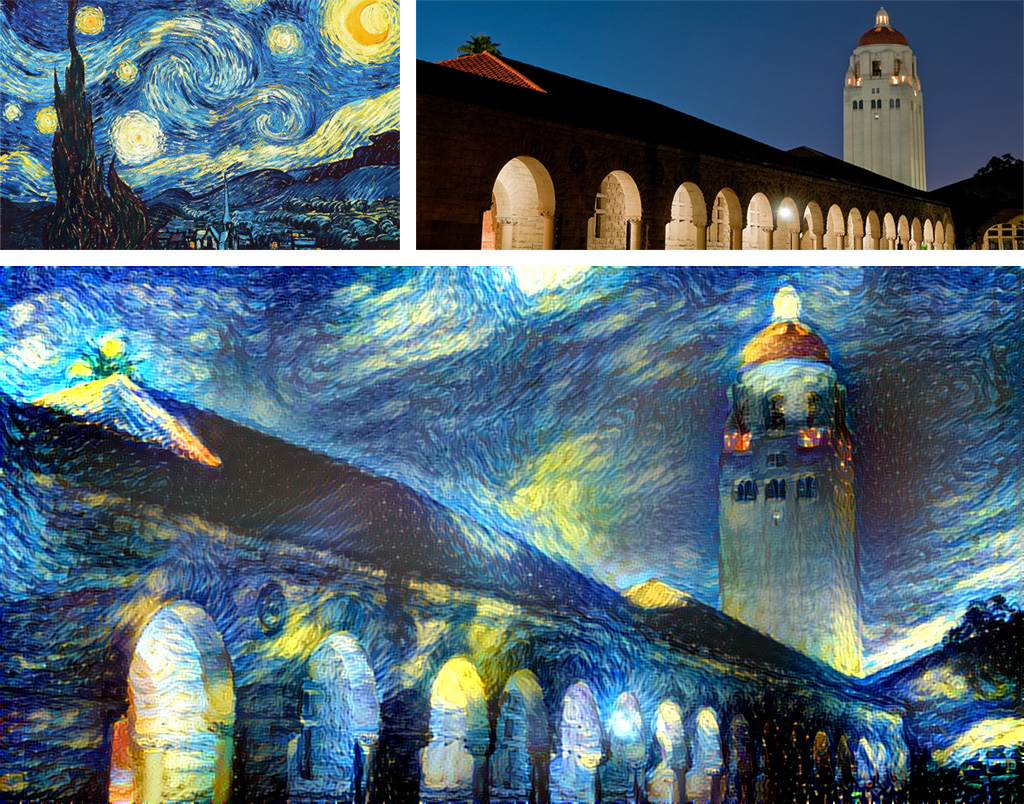
\includegraphics[width=\textwidth]{gfx/neural-style-composed}
  \caption{
  Neural Style algorithm implementation \cite{Johnson2015} results.
  \textbf{Top-left}: \textit{The Starry Night} by Vincent van Gogh, 1889, source of style.
  \textbf{Top-right}: Night-time photograph of the Stanford campus, source of content.
  \textbf{Bottom}: Combination of style and content from the images above.
  }
  \label{fig:sec:intro:neural-style}
\end{figure}

The problem of the separation of style and content, however, has barely been tackled explicitly in pattern recognition \cite{Karayev2014}.
Neither deep neural networks trained for pattern recognition are, in any way, designed for separating style and content, as their goal is to simply classify input correctly.
Surprisingly, they seem to acquire an innate understanding of the notions of style and content in the process, as it became clear in \citeauthor{Gatys2015B}'s research \cite{Gatys2015B}.

\citeauthor{Gatys2015B} developed an algorithm capable of blending the style and content of two source images into a new one, this way effectively providing a holistic approach to a long-standing problem.
Instead of using a deep neural network trained for that precise purpose, the algorithm utilizes a network already trained for object recognition and, as the network processes an image, its content and style are extracted separately from the intermediate layers.
\autoref{fig:sec:intro:neural-style} shows the results from the style transfer capabilities of Neural Style \cite{Gatys2015B}.

These uncanny findings open the door for wondering about other underlying understanding deep neural networks may develop as side effects of a training process, how this can be used to better understand the human brain \cite{Yamins2016}, or what other applications similar methods can achieve.


% ------------------------------------------------------------------------------

\section{Goals}
\label{sec:intro:goals}

This thesis focuses on \citeauthor{Gatys2015B}'s Neural Style algorithm \cite{Gatys2015B} and its novel approach for separating style and content from the optic of deep neural networks.
Being the field of Artificial Neural Networks extensive and in constant revision, in an effort to stay on topic the scope of our work has been restricted to the following goals:

\begin{enumerate}
  \item Studying the motivation and challenges of the separation of style and content.
  \item Reviewing traditional approaches for the separation of style and content.
  \item Understanding Neural Style's approach for separating style and content.
  \item Exploring the conditions that enabled the development of Neural Style.
  \item Reflecting on the impact of methods applied in Neural Style.
  \item Finding novel applications that apply said methods.
  \item Proposing future work in the same line of research.
\end{enumerate}


% ------------------------------------------------------------------------------

\section{Thesis Structure}
\label{sec:intro:structure}

This document covers the outcome of the goals previously stated as well as the necessary theoretical background to fully comprehend it, and the structure is as follows.

\begin{minipage}{\textwidth}
  \textbf{\nameref{chap:theory}} \\[0.2em]
  In Chapter~\ref{chap:theory} we give a theoretical introduction on artificial neural networks and Deep Learning as well as the general concepts used in particular implementations of networks that will be used in later chapters to further discuss separation of style and content.
\end{minipage}

\begin{minipage}{\textwidth}
  \textbf{\nameref{chap:context}} \\[0.2em]
  In Chapter~\ref{chap:context} we introduce the context that led to the successful separation of style and content with deep neural networks. We cover advances in object recognition, newly developed methods to visualize the internal representations in deep neural networks, and some background on the task of style transfer.
\end{minipage}

\begin{minipage}{\textwidth}
  \textbf{\nameref{chap:system}} \\[0.2em]
  In Chapter~\ref{chap:system} we present and discuss Neural Style \cite{Gatys2015B}, an algorithm that successfully separates content and style by using a deep neural network trained for object recognition.
\end{minipage}

\begin{minipage}{\textwidth}
  \textbf{\nameref{chap:applications}} \\[0.2em]
  In Chapter~\ref{chap:applications} we review some of the new applications triggered by Neural Style as well as novel techniques using similar approaches with deep neural networks for perceptually challenging tasks.
\end{minipage}

\begin{minipage}{\textwidth}
  \textbf{\nameref{chap:conclusion}} \\[0.2em]
  Finally, in Chapter~\ref{chap:conclusion} we propose future work based on concepts and ideas triggered by the Neural Style approach, aiming beyond the separation of style and content into the study of algorithmic aesthetics.
\end{minipage}
